\documentclass{article}
\usepackage{iclr2026_conference,times}

\usepackage{amsmath,amssymb,amsfonts,amsthm,mathtools}
\usepackage[utf8]{inputenc}
\usepackage[T1]{fontenc}
\usepackage{hyperref}
\usepackage{url}
\usepackage{booktabs}
\usepackage{nicefrac}
\usepackage{microtype}
\usepackage{xcolor}
\usepackage{graphicx}
\usepackage{subcaption}
\usepackage{multirow}
\usepackage{algorithm}
\usepackage{algorithmic}
\usepackage[capitalize,noabbrev]{cleveref}

\theoremstyle{plain}
\newtheorem{theorem}{Theorem}[section]
\newtheorem{proposition}[theorem]{Proposition}
\newtheorem{lemma}[theorem]{Lemma}
\newtheorem{corollary}[theorem]{Corollary}
\theoremstyle{definition}
\newtheorem{definition}[theorem]{Definition}
\newtheorem{assumption}[theorem]{Assumption}
\theoremstyle{remark}
\newtheorem{remark}[theorem]{Remark}

\crefname{assumption}{Assumption}{Assumptions}
\Crefname{assumption}{Assumption}{Assumptions}

\newcommand{\R}{\mathbb{R}}
\newcommand{\E}{\mathbb{E}}
\DeclareMathOperator*{\argmax}{arg\,max}
\DeclareMathOperator*{\argmin}{arg\,min}
\newcommand{\ctx}{\mathrm{ctx}}
\newcommand{\kv}{\mathrm{kv}}
\newcommand{\pim}{\mathrm{pim}}
\newcommand{\gpu}{\mathrm{gpu}}
\newcommand{\speedup}{\mathrm{speedup}}
\newcommand{\oracle}{\mathrm{oracle}}
\newcommand{\online}{\mathrm{online}}


\title{When Does Virtual PIM Help LLM Decoding?\\
A Trace-Driven Characterization of Regime Entry and KV-Related Decision Signals}

\author{Anonymous Authors}

\begin{document}

\maketitle

\begin{abstract}
Large language model (LLM) decoding contains a mix of compute-sensitive and memory-sensitive regions, which makes processing-in-memory (PIM) style offloading potentially attractive. The practical difficulty is that offload value is highly condition-dependent: some decode runs benefit substantially, while others do not. We present a trace-driven framework for studying \emph{virtual} PIM decision signals during LLM decoding. Our approach collects runtime-grounded decode traces from open-source stacks, attaches a prior-work-grounded virtual PIM cost model, and evaluates static and dynamic scheduling rules without claiming real hardware speedups. Using CPU and GPU traces across older GPT-style models and newer 4-bit instruct models, we find a consistent weak-signal versus positive-signal split: short-context decoding often shows no realistic gain, while longer-context decoding repeatedly becomes favorable for dynamic offload. Dense context sweeps show that context length is the clearest coarse regime-entry variable in our current setup, but the onset differs across model families. We further show that explicit KV-cache pressure proxies are more consistent with the observed boundary than a static attention heuristic alone, and that KV-aware features can help recover some early-positive families that a generic realistic feature policy misses. These results position virtual PIM not as a uniformly beneficial accelerator, but as a regime-dependent opportunity whose value can be characterized from runtime traces.

\end{abstract}

\section{Introduction}

Large language model (LLM) decoding is increasingly limited by data movement rather than raw arithmetic throughput, especially as context length grows and KV-cache traffic expands. This has renewed interest in processing-in-memory (PIM) style acceleration for inference. Recent PIM and near-memory systems papers show that decode workloads can expose kernels with different bottleneck types, which suggests that dynamic offloading may matter. However, an important question remains underexplored: \emph{when does virtual PIM offloading actually become worthwhile during decoding, and what signal best predicts regime entry?}

This question is easy to ask but difficult to answer cleanly. Real PIM-enabled heterogeneous systems are expensive to build, production LLM serving stacks hide many low-level details, and performance conclusions are sensitive to workload regime. As a result, it is difficult to separate three issues: whether offload value is real at all, which runtime conditions trigger it, and whether simple heuristics such as ``offload attention'' are sufficient to detect those conditions.

We study this problem using a trace-driven virtual PIM evaluation framework for LLM decoding. Our framework instruments open-source decoding runs, extracts region-level traces and runtime features, and replays them through a prior-work-grounded virtual PIM cost model. This lets us evaluate static and dynamic decision rules on real decode behavior while explicitly avoiding direct hardware-speedup claims. The goal is not to introduce a new PIM architecture, but to characterize the operating regimes in which PIM-style offloading appears useful and the runtime signals that best predict those regimes under a transparent virtual backend.

The central empirical result is a consistent weak-signal versus positive-signal split. Short-context decoding often shows no realistic gain even when an oracle policy still has latent upside, which means the framework is not fabricating benefits everywhere. In contrast, longer-context decoding repeatedly enters a positive offload regime. Dense context sweeps sharpen this transition and show that context length is the clearest coarse regime-entry variable in our current setup, but the onset is model-family dependent. For example, \texttt{Qwen2.5-1.5B} shows delayed onset, while \texttt{Qwen3-8B}, \texttt{SmolLM2-1.7B}, and \texttt{Phi-3.5-mini} enter the positive regime earlier. We further find that KV-cache-related signals are more consistent with the observed boundary than attention labels alone, but we treat this as predictive evidence rather than as a causal proof.

\begin{figure}[t]
    \centering
    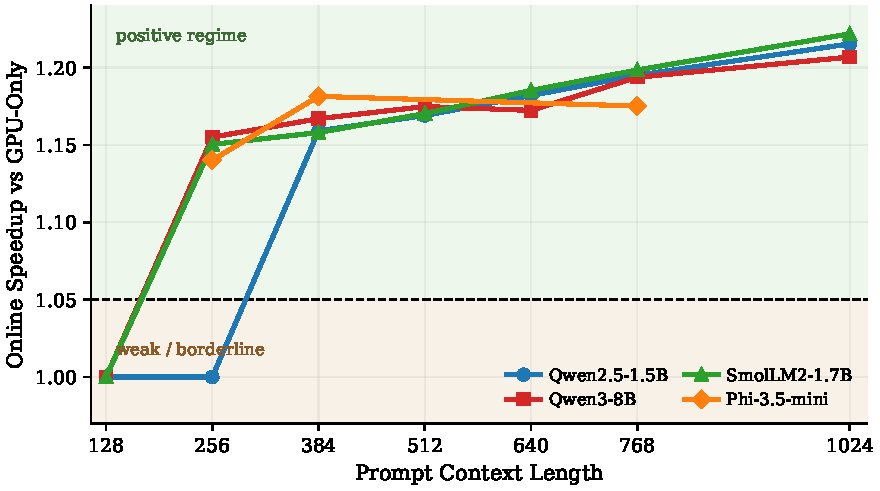
\includegraphics[width=0.95\linewidth]{figures/final_figures/paper_backbone_context_transition.pdf}
    \caption{Dense context sweeps show that virtual PIM benefit is regime-dependent rather than universal. In our current setup, context length is the clearest coarse regime-entry variable, but onset is family-dependent: \texttt{Qwen2.5-1.5B} enters later than \texttt{Qwen3-8B}, \texttt{SmolLM2-1.7B}, and \texttt{Phi-3.5-mini}.}
    \label{fig:context-transition}
\end{figure}

These observations lead to a narrower and safer policy message than ``dynamic scheduling is better.'' A static attention heuristic is directionally useful, but it is too permissive. A generic realistic feature policy is also too conservative in several important cases. In contrast, KV-aware features can help refine boundary detection in some early-positive families, which suggests that the core decision problem is not merely to identify attention regions, but to detect when a decode stream has plausibly crossed into a positive offload regime.

Our contribution is therefore an empirical systems characterization rather than a hardware paper. We do not claim real PIM speedups, cycle-accurate backend fidelity, or a final deployment-ready scheduler. Instead, we make the following contributions:

\begin{itemize}
\item We present a trace-driven framework for studying virtual PIM decision signals during LLM decoding using runtime-grounded traces, a transparent virtual PIM backend, and policy replay.
\item We show that virtual PIM value is regime-dependent: short-context decoding is often weak or borderline, while longer-context decoding repeatedly enters a positive offload regime.
\item We show that context length is the clearest coarse regime-entry variable in our current setup, but that the onset of positive offload value is model-family dependent.
\item We show that the observed boundary is consistent with explicit KV-cache pressure proxies, and that KV-aware features can complement coarse context cues for positive-regime detection.
\end{itemize}

The rest of the paper is organized as follows. \Cref{sec:related} positions this work relative to prior PIM, KV-cache, and scheduling systems. \Cref{sec:method} describes the trace-driven framework and the evaluation protocol. \Cref{sec:experiments} presents the regime characterization, mechanism evidence, and policy analysis. \Cref{sec:conclusion} concludes with limitations and future directions.

\section{Related Work}
\label{sec:related}

\paragraph{PIM and heterogeneous acceleration for LLM inference.}
Recent systems work argues that LLM decoding contains kernels with heterogeneous bottlenecks and that PIM or near-memory execution can improve performance in the right regimes. PAPI is the closest direct prior in spirit: it studies dynamic kernel assignment for LLM decoding on a PIM-enabled heterogeneous system and shows that static mapping is insufficient in the presence of dynamic parallelism \citep{he2025papi}. Other architecture papers such as PIM Is All You Need and CENT push the argument further by proposing concrete PIM-enabled or GPU-free systems for LLM inference \citep{gu2025pim,wang2025cent}. These papers are important because they motivate why PIM may matter at decode time. Our work differs in scope and claim boundary. We do not propose a new PIM architecture or claim real hardware speedups. Instead, we use runtime-grounded traces and a virtual backend to characterize \emph{when} PIM-style offloading appears useful and which runtime signals best predict regime entry under that backend.

\paragraph{KV-cache-centric inference systems.}
Another closely related line of work treats the KV cache as the central systems bottleneck in long-context inference. Mooncake, for example, proposes a KVCache-centric disaggregated serving architecture and scheduler for long-context LLM service \citep{qin2025mooncake}. Other work studies dynamic KV-cache placement or online scheduling under heterogeneous memory constraints \citep{akhauri2025kvplacement,microsoft2025kvscheduling}. These papers substantially overlap with our mechanism story: KV traffic and memory pressure matter. However, they ask a different question. Their main objective is serving architecture, memory placement, or online scheduling under explicit storage constraints, whereas our focus is a trace-driven characterization of virtual PIM offload regimes during decoding. In particular, we ask whether KV-related signals provide better predictive support for positive-regime detection than a static attention rule.

\paragraph{LLM inference scheduling and serving optimization.}
Constraint-aware and throughput-aware LLM schedulers also provide important context. ExeGPT studies resource scheduling for LLM inference under latency constraints and shows that execution configuration should adapt to workload characteristics \citep{oh2024exegpt}. These works support the broader view that LLM inference should be treated as a scheduling problem rather than a fixed execution template. Our policy analysis is aligned with that perspective, but we focus on a narrower issue: not the entire serving system, but the emergence of positive virtual PIM offload regimes at decode time. This is why our analysis emphasizes regime entry, negative short-context cases, and runtime signals such as memory pressure proxy rather than only throughput-oriented scheduler optimization.

\paragraph{Trace-driven and simulation-based LLM evaluation.}
A growing body of work uses simulation or replay to study LLM inference systems without rebuilding full production stacks. This makes trace-driven methodology itself a crowded space, which means our novelty does not come from using simulation alone. Our contribution is instead the combination of runtime-grounded decode traces, a PIM-specific virtual what-if backend, and an empirical finding: the onset of virtual offload value is context-sensitive, model-family dependent, and only partially captured by static attention labels. We therefore position the paper as an empirical characterization and decision-signal study enabled by a trace-driven framework, rather than as a general LLM simulator paper.

\section{Trace-Driven Virtual PIM Evaluation}
\label{sec:method}

\subsection{Problem Framing}

We study virtual PIM offloading during autoregressive LLM decoding. Let a decode trace be a sequence of region-level records
\[
\mathcal{T} = \{r_t\}_{t=1}^{T},
\]
where each record contains a region identity, measured latency, estimated bytes moved, arithmetic intensity, context length, batch size, and auxiliary metadata derived from the runtime. We do not attempt to model a full physical PIM system. Instead, we use these records to evaluate a virtual decision problem: for each decode region, should execution remain on the GPU or be offloaded to a hypothetical PIM backend under a prior-work-grounded latency model?

\subsection{Trace Collection}

Our framework instruments real decoding runs from open-source runtimes and collects region-level records for attention and MLP-dominated portions of each decode step. Each trace record stores:
\begin{itemize}
\item measured latency,
\item estimated floating-point work and bytes moved,
\item current context length and batch size,
\item runtime-derived KV-related proxies such as $\kv$ bytes and memory pressure.
\end{itemize}
This design gives us a runtime-grounded description of decode behavior without requiring proprietary serving stacks or custom hardware counters.

\subsection{Virtual PIM Backend}

The virtual backend is intentionally transparent. It uses a prior-work-grounded cost model rather than a cycle-accurate microarchitecture. The GPU-side assumptions are anchored to a roofline-style A100 reference, while the PIM side is parameterized by bandwidth, compute throughput, and fixed orchestration overheads. This makes the backend suitable for trace-grounded replay, signal comparison, and sensitivity analysis, but not for direct hardware-speedup claims.

For each trace record $r$, the GPU latency estimate is
\[
L_{\mathrm{gpu}}(r)=
\begin{cases}
\ell_{\mathrm{trace}}(r), & \text{if measured region latency is available}, \\
\max\!\left(\frac{\mathrm{FLOPs}(r)}{\Theta_{\mathrm{gpu}}}, \frac{\mathrm{Bytes}(r)}{B_{\mathrm{gpu}}}\right), & \text{otherwise}.
\end{cases}
\]
The virtual PIM latency uses the trace-grounded GPU latency as an anchor and then rescales its compute- and memory-dominant shares:
\[
L_{\mathrm{pim}}(r)=
\max\!\left(
L_{\mathrm{gpu}}(r)\cdot s_c(r)\cdot \frac{\Theta_{\mathrm{gpu}}}{\Theta_{\mathrm{pim}}^{\mathrm{eff}}(r)},
L_{\mathrm{gpu}}(r)\cdot s_m(r)\cdot \frac{B_{\mathrm{gpu}}}{B_{\mathrm{pim}}^{\mathrm{eff}}(r)}
\right)
\;+\;
\tau_{\mathrm{transfer}}
\;+\;
\tau_{\mathrm{sync}},
\]
where $s_c(r)$ and $s_m(r)$ are the compute- and memory-share terms derived from the GPU roofline decomposition. For attention regions, $B_{\mathrm{pim}}^{\mathrm{eff}}(r)$ receives a context-scaled bandwidth bonus; for non-attention and MLP regions, $\Theta_{\mathrm{pim}}^{\mathrm{eff}}(r)$ is reduced by fixed penalties to reflect their weaker fit to memory-centric execution. The default parameters and provenance split are summarized in \Cref{tab:backend-measured-modeled,tab:backend-params}.

\begin{table}[t]
\centering
\caption{Virtual backend inputs grouped by provenance.}
\label{tab:backend-measured-modeled}
\begin{tabular}{p{0.22\linewidth}p{0.37\linewidth}p{0.27\linewidth}}
\toprule
Category & Fields & Source / Interpretation \\
\midrule
Trace-measured & region label, measured latency, context length, batch size & Directly observed in the collected decode traces \\
Trace-derived & bytes moved, FLOPs, arithmetic intensity, estimated KV bytes, KV bytes/token, memory-pressure proxy & Derived from runtime metadata and trace-side estimators \\
Modeled only & roofline compute/memory shares, effective PIM bandwidth/throughput modifiers, transfer/sync overheads, estimated PIM latency & Virtual replay assumptions used only for what-if comparison \\
\bottomrule
\end{tabular}
\end{table}

\begin{table}[t]
\centering
\caption{Default virtual backend parameters, role, and provenance.}
\label{tab:backend-params}
\begin{tabular}{p{0.28\linewidth}p{0.13\linewidth}p{0.24\linewidth}p{0.24\linewidth}}
\toprule
Parameter & Default & Role & Provenance \\
\midrule
GPU peak BW & 1935 GB/s & Roofline anchor for memory time & Prior-work A100-style roofline anchor \\
GPU peak throughput & 312 TFLOP/s & Roofline anchor for compute time & Prior-work A100-style roofline anchor \\
PIM peak BW & 2400 GB/s & Baseline virtual PIM memory rate & Memory-centric default: modestly above GPU BW to encode bandwidth advantage without assuming equal compute \\
PIM peak throughput & 18 TFLOP/s & Baseline virtual PIM compute rate & Conservative low-throughput default to avoid overstating compute-heavy gains \\
Transfer overhead & 0.020 ms & Per-dispatch orchestration cost & Conservative midpoint varied again in preset sensitivity \\
Sync overhead & 0.010 ms & Per-dispatch synchronization cost & Conservative midpoint varied again in preset sensitivity \\
Attention BW bonus & 0.20 & Long-context attention memory modifier & Qualitative prior reflecting stronger KV pressure at long context \\
FC parallelism penalty & 0.25 & MLP parallelism penalty & Deliberate penalty to avoid overstating non-attention and MLP benefit \\
Non-attention penalty & 0.10 & Throughput penalty outside attention & Deliberate penalty to keep non-attention gains conservative \\
\bottomrule
\end{tabular}
\end{table}


This paper treats the virtual backend as a methodological enabler rather than as the main novelty. All central claims are therefore phrased in terms of regime characterization and relative policy behavior, not exact hardware performance.

\subsection{Policies}

We evaluate the following policy families:
\begin{itemize}
\item \textbf{GPU-only}: never offload.
\item \textbf{Static attention}: offload all attention regions.
\item \textbf{Online predictor}: a lightweight dynamic predictor using runtime features.
\item \textbf{Adaptive feature}: a realistic feature-based policy using context, bytes moved, arithmetic intensity, latency, and region bias.
\item \textbf{KV regime}: a realistic policy that augments runtime features with explicit KV-related signals such as estimated $\kv$ bytes, $\kv$ bytes per token, and memory pressure proxy.
\item \textbf{Oracle}: an upper bound that chooses the lower-cost device for each record under the virtual backend.
\end{itemize}

The key comparison in this paper is not between a sophisticated learned scheduler and a naive baseline, but between different kinds of realistic decision signals. We use this comparison to test whether static attention rules are sufficient, whether context length alone is already a strong coarse cue, and whether explicit KV-related signals provide complementary information near the regime boundary.

\subsection{Claims and Evaluation Logic}

Our experimental logic follows three questions.
\begin{enumerate}
\item \textbf{Regime characterization}: when does realistic dynamic offload show positive value, and when does it fail?
\item \textbf{Predictive signals}: is the transition more consistent with context alone, attention share, or KV-related pressure signals?
\item \textbf{Decision implication}: do static attention rules and generic realistic heuristics over- or under-predict early-positive cases, and can KV-aware features refine the boundary?
\end{enumerate}

These questions motivate the main figures and tables in the paper. \Cref{fig:context-transition} addresses the first question, \Cref{fig:kv-pressure} and \Cref{fig:decision-signal-study} address the second, and \Cref{fig:policy-comparison} provides a focused case-study view for the third.

\section{Experiments}
\label{sec:experiments}

\subsection{Setup}

We evaluate the framework on CPU and GPU traces collected from older GPT-style models and newer 4-bit instruct families. The strongest modern-family evidence comes from dense context sweeps on \texttt{Qwen2.5-1.5B}, \texttt{Qwen3-8B}, and \texttt{SmolLM2-1.7B}, together with an additional \texttt{Phi-3.5-mini} validation. Across the current artifact set, the main analysis covers 30 workload points. We report speedup relative to GPU-only execution under the virtual backend. Our primary realistic baselines are \texttt{online\_predictor}, \texttt{adaptive\_feature}, and \texttt{kv\_regime}; \texttt{oracle} serves only as an upper bound.

\subsection{Backend Transparency and Sensitivity}

The largest methodological risk in this paper is over-interpreting a virtual backend. We therefore make the backend explicit. \Cref{tab:backend-measured-modeled} separates trace-measured, trace-derived, and modeled quantities, while \Cref{tab:backend-params} lists the default parameters used by the virtual replay model. The most important anchor is that measured trace latency is used directly as the GPU reference whenever available; the roofline terms are then used only to decompose that measured latency into compute- and memory-dominant shares before applying the virtual PIM rescaling.

The sensitivity analysis is defensive but important. Conservative, default, and optimistic virtual-PIM presets change absolute speedups, but the canonical weak cases remain weak and the canonical long-context positive cases remain positive. We therefore treat the backend as a transparent what-if model whose main value lies in preserving regime ordering and relative decision-signal comparisons rather than exact numerical speedup claims.

\subsection{Negative Results Matter}

A key result of this study is that virtual PIM value is not automatic. \Cref{fig:negative-cases} shows this as a distribution rather than as a handful of cherry-picked bars. The left panel shows a clear mass of workloads near $\online = 1.0\times$, while the right panel shows that only $3/9$ short-context workloads are online-positive. The fraction rises to $9/9$ for mid-context workloads and $12/12$ for long-context workloads.

These negative results are important because they improve credibility. Rather than showing gains everywhere, the framework separates weak and positive regimes at the workload-distribution level, which makes the later positive-regime evidence more trustworthy. This also clarifies the main scientific claim: virtual PIM offload becomes interesting only after the decode stream enters the right operating regime, and short-context execution often fails to provide that signal.

\begin{figure}[t]
    \centering
    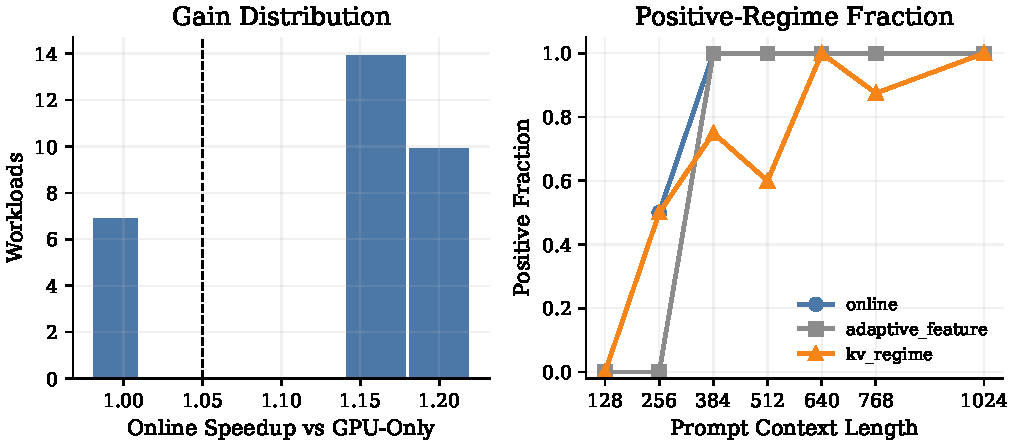
\includegraphics[width=0.95\linewidth]{figures/final_figures/paper_negative_cases.pdf}
    \caption{Distributional negative-result evidence. Left: workload-level distribution of realistic online gains. Right: positive-regime fraction versus context. Gains do not appear automatically, and short-context workloads are much more often weak.}
    \label{fig:negative-cases}
\end{figure}

\subsection{Context Governs Regime Entry}

\Cref{fig:context-transition} is the best-supported empirical result in the paper. It sharpens the regime transition using dense context sweeps instead of only coarse points such as 256, 512, and 768. The delayed-onset \texttt{Qwen2.5-1.5B} family transitions from weak to positive between 256 and 384 tokens, while \texttt{Qwen3-8B} and \texttt{SmolLM2-1.7B} become positive earlier, between 128 and 256 tokens. The extra \texttt{Phi-3.5-mini} validation remains positive at 256, 384, and 768 tokens, which shows that early-positive behavior is not isolated to a single family.

This result matters for two reasons. First, it supports a stronger claim than ``longer context helps'': in our current setup, context length is the clearest \emph{coarse} regime-entry variable. Second, it shows that onset is family-dependent rather than universal, which implies that a global rule such as ``offload attention after context 512'' is too coarse.

\subsection{KV-Related Signals Are Predictive, Not Causal}

\begin{figure}[t]
    \centering
    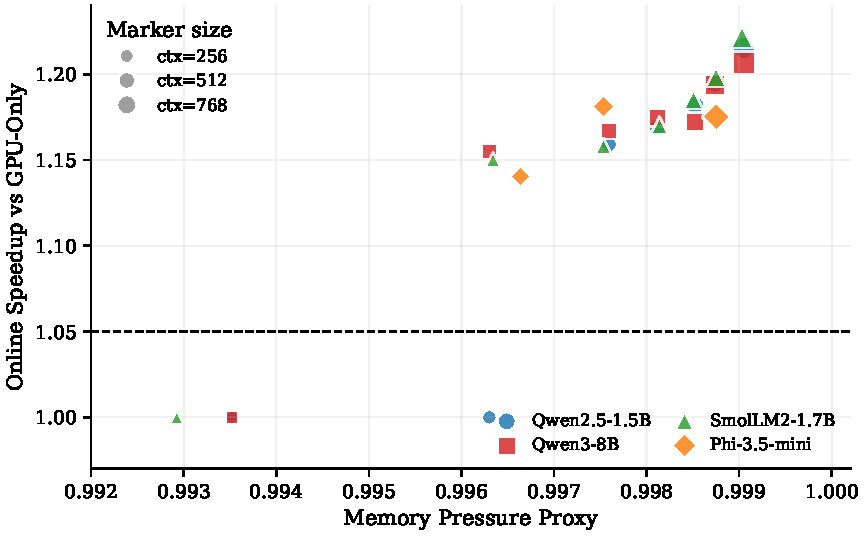
\includegraphics[width=0.95\linewidth]{figures/final_figures/paper_backbone_kv_pressure_vs_speedup.pdf}
    \caption{Higher memory-pressure proxy values align with positive online speedup across modern families. The figure is consistent with a KV-centered mechanism, but should be interpreted as predictive evidence rather than as causal proof.}
    \label{fig:kv-pressure}
\end{figure}

The mechanism analysis strengthens the paper beyond a context-only observation, but we intentionally stop short of a causal claim. Across the focused GPU suite, higher memory-pressure proxy values align with positive online speedup more directly than attention share alone. We therefore interpret the evidence as follows: the observed regime boundary is consistent with rising KV-cache-related pressure, and KV-related proxies are useful predictive correlates under the current backend.

This view also helps account for family-dependent onset. Different families can exhibit different KV-cache traffic profiles and attention behavior under similar context lengths, which means the same context value need not imply the same offload regime boundary.

\subsection{Held-Out Decision-Signal Study}

To test signal quality more directly, we built a workload-level classifier for positive-regime detection, where the label is whether the realistic online predictor reaches $\mathrm{speedup} > 1.05\times$. We compare five signal families: attention-only, context-only, context+attention, KV-only, and all-features, using family-held-out and context-bucket-held-out splits.

The result is more nuanced than our earlier draft suggested. On family-held-out splits, context-only is the strongest coarse detector (F1 $=0.936$, false-positive rate $=0.000$), while attention-only is too permissive (positive recall $=0.944$, false-positive rate $=0.667$). On context-bucket-held-out splits, the all-feature detector is strongest overall (F1 $=0.767$ versus $0.738$ for context-only), which suggests that KV-related signals are complementary decision aids rather than a standalone dominant mechanism.

\begin{figure}[t]
    \centering
    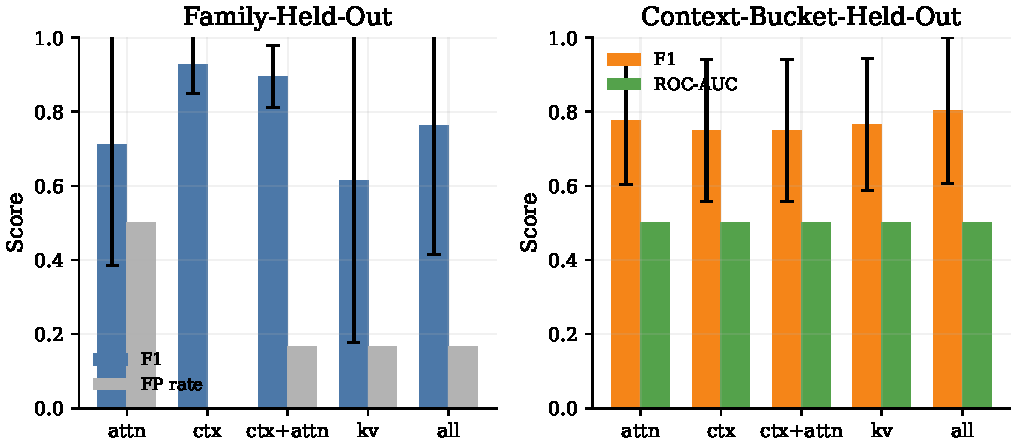
\includegraphics[width=0.95\linewidth]{figures/final_figures/paper_decision_signal_study.pdf}
    \caption{Held-out decision-signal study for workload-level positive-regime detection. Attention-only cues over-predict positive regimes, context is the strongest coarse predictor in the current setup, and all-feature detectors modestly improve context-bucket-held-out detection.}
    \label{fig:decision-signal-study}
\end{figure}

\subsection{Policy Case Study}

The policy results still matter, but they should be read as a focused case study rather than as proof of a universally best scheduler. A static attention heuristic is directionally useful, but it remains too permissive. The generic realistic policy \texttt{adaptive\_feature} is safer overall, but it misses several early-positive cases such as \texttt{Qwen3 @ ctx256}, \texttt{SmolLM2 @ ctx256}, and \texttt{Phi-3.5 @ ctx256}.

The more defensible message is that explicit KV-aware features can matter on some early-positive families. \texttt{kv\_regime} recovers \texttt{Qwen3 @ ctx256}, \texttt{SmolLM2 @ ctx256}, and \texttt{Phi-3.5 @ ctx256} without relying on oracle-like cost-model internals, but it is not uniformly dominant on every boundary point. We therefore frame this result as an existence proof that KV-aware decision features can be useful, not as a final scheduler contribution.

\begin{figure}[t]
    \centering
    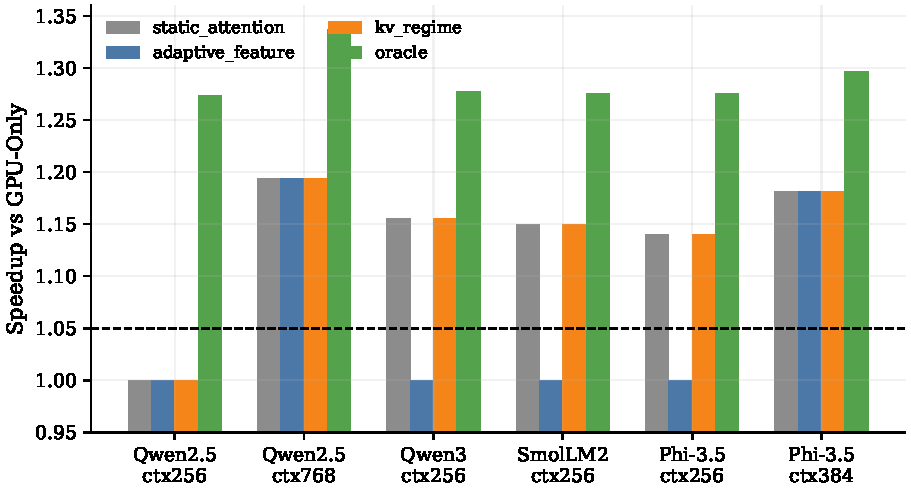
\includegraphics[width=0.95\linewidth]{figures/final_figures/paper_policy_comparison.pdf}
    \caption{Focused policy case study on selected early-positive workloads. KV-aware decision features can recover some early-positive cases that a generic realistic policy misses, but the figure should not be read as a universal ranking over all workloads.}
    \label{fig:policy-comparison}
\end{figure}

The policy comparison makes the paper's systems implication more concrete. Static attention offloading is often useful, but it does not capture why early-positive modern families differ from delayed-onset ones. The generic realistic policy \texttt{adaptive\_feature} is safer overall, but it still misses important early-positive points. In contrast, \texttt{kv\_regime} recovers several of these cases using only runtime-style KV-related signals and without direct oracle-like cost-model internals.

\subsection{Batch and Robustness Are Defensive Evidence}

The controlled batch study shows that batch is weaker than context in our current setup. On \texttt{Qwen2.5-1.5B}, online speedup remains exactly $1.000\times$ across $bs \in \{1,2,4,8\}$ at context 256, while remaining positive but nearly flat ($1.186\times$ to $1.194\times$) across the same batch sweep at context 768. Batch therefore changes magnitude within a regime more than it changes the regime itself.

The cost-model sensitivity analysis serves as a robustness check. Conservative, default, and optimistic virtual-PIM presets change absolute speedup numbers, but the canonical weak cases remain weak and the canonical long-context positive cases remain positive. Early-onset short-context points are closer to the decision boundary, but the main long-context story is stable. These results make the paper less vulnerable to the criticism that the conclusions are artifacts of a single narrow virtual backend setting.

\subsection{Summary of Experimental Takeaways}

Taken together, the experiments support four claims. First, virtual PIM value is regime-dependent rather than universal. Second, context length is the clearest coarse regime-entry variable in our current study. Third, the onset of positive offload value varies across model families. Fourth, KV-aware signals provide complementary predictive information near the boundary, while static attention labels alone are too permissive.

\section{Conclusion}
\label{sec:conclusion}

We presented a trace-driven framework for studying virtual PIM decision signals during LLM decoding and used it to characterize when offload value appears. The main conclusion is not that PIM-style offloading always helps, but that it becomes worthwhile only after the decode stream enters the right operating regime. In our current experiments, context length is the clearest coarse regime-entry variable, the onset is model-family dependent, and the transition is more consistent with rising KV-cache pressure than with static attention labels alone. KV-aware features therefore look useful as complementary decision signals, especially near early-positive boundary cases.

The project has important limitations. Our backend is prior-work-grounded but still virtual rather than cycle-accurate, so we do not claim real hardware speedups. Our traces come from open-source runtimes rather than production serving engines, and our model set, while broader than the initial study, still does not cover very large serving-scale models. We therefore view the paper as an empirical characterization study rather than a final accelerator or scheduler paper.

The most useful next steps are to add a stronger runtime-diversity check, obtain at least one hardware or emulation anchor point for the virtual backend, and test whether the family-dependent onset patterns persist under broader serving conditions such as continuous batching.


\bibliography{references}
\bibliographystyle{iclr2026_conference}

\newpage
\appendix
\section{Additional Details}

\subsection{Framework Overview}

The end-to-end workflow is: real decode run $\rightarrow$ trace adapter $\rightarrow$ region-level trace $\rightarrow$ virtual PIM replay $\rightarrow$ policy comparison. The framework deliberately separates runtime measurement from the virtual backend so that different cost-model settings can be replayed on the same collected traces.

\subsection{Additional Tables}

Table~\ref{tab:main-modern-results} summarizes representative modern-family results, and Table~\ref{tab:family-onset} summarizes the first positive context by family.

\begin{table}[t]
\centering
\caption{Representative regime-transition results on modern 4-bit instruct models.}
\label{tab:main-modern-results}
\begin{tabular}{lcccc}
\toprule
Model & Context & Online & KVRegime & Oracle \\
\midrule
Qwen2.5-1.5B & 256 & 1.000 & 1.000 & 1.274 \\
Qwen2.5-1.5B & 512 & 1.169 & 1.169 & 1.306 \\
Qwen3-8B & 256 & 1.155 & 1.155 & 1.277 \\
SmolLM2-1.7B & 256 & 1.150 & 1.150 & 1.276 \\
Phi-3.5-mini & 256 & 1.140 & 1.140 & 1.276 \\
Phi-3.5-mini & 384 & 1.181 & 1.181 & 1.297 \\
\bottomrule
\end{tabular}
\end{table}

\begin{table}[t]
\centering
\caption{Family-dependent onset of the positive offload regime.}
\label{tab:family-onset}
\begin{tabular}{lc}
\toprule
Family & First online-positive context \\
\midrule
gpt2 & 512 \\
opt-125m & 512 \\
Qwen2.5-1.5B & 384 \\
Qwen3-8B & 256 \\
SmolLM2-1.7B & 256 \\
Phi-3.5-mini & 256 \\
\bottomrule
\end{tabular}
\end{table}


\subsection{Robustness Notes}

The sensitivity study changes PIM bandwidth and latency presets while leaving the decode traces fixed. The most robust conclusion is the long-context positive-regime story. Borderline early-onset short-context points are more parameter-sensitive, which is why the main paper phrases them as family-dependent onset evidence rather than as universal short-context gains.

\subsection{Reproducibility}

All main figures in the paper are generated from reproducible scripts and stored under the project \texttt{final/} package. The trace schema, simulator, cost model, and policy implementations are contained in the repository. The paper focuses on runtime-grounded virtual replay rather than private serving traces or proprietary hardware measurements.


\end{document}
